%%%%%%%%%%%%%%%%%%%%%%%%%%%%%%%%%%%%%%%%%
% Thin Sectioned Essay
% LaTeX Template
% Version 1.0 (3/8/11)
%
% This template has been downloaded from:
% http://www.LaTeXTemplates.com
%
% Original Author:
% Nicolas Diaz (nsdiaz@uc.cl) with extensive modifications by:
% Vel (vel@latextemplates.com)
%
% License:
% CC BY-NC-SA 3.0 (http://creativecommons.org/licenses/by-nc-sa/3.0/)
%
%%%%%%%%%%%%%%%%%%%%%%%%%%%%%%%%%%%%%%%%%

%----------------------------------------------------------------------------------------
%	PACKAGES AND OTHER DOCUMENT CONFIGURATIONS
%----------------------------------------------------------------------------------------

\documentclass[a4paper, 11pt]{article} % Font size (can be 10pt, 11pt or 12pt) and paper size (remove a4paper for US letter paper)
\usepackage{hyperref}

\usepackage[protrusion=true,expansion=true]{microtype} % Better typography
\usepackage{graphicx} % Required for including pictures
\usepackage{wrapfig} % Allows in-line images
\usepackage{tablefootnote} % to display footnotes in tables
\usepackage{threeparttable}
\usepackage[toc,page]{appendix}
\usepackage{multirow}
\usepackage{color}

\usepackage{mathpazo} % Use the Palatino font
\usepackage[T1]{fontenc} % Required for accented characters
\linespread{1.05} % Change line spacing here, Palatino benefits from a slight increase by default

\newcommand{\hls}{HLS\,J0918+5142}
\makeatletter
%\renewcommand\@biblabel[1]{\textbf{#1.}} % Change the square brackets for each bibliography item from '[1]' to '1.'
\renewcommand{\@listI}{\itemsep=0pt} % Reduce the space between items in the itemize and enumerate environments and the bibliography

\renewcommand{\maketitle}{ % Customize the title - do not edit title and author name here, see the TITLE block below
\begin{flushleft} % Right align
{\LARGE\@title} % Increase the font size of the title

\vspace{50pt} % Some vertical space between the title and author name

{\large\@author} % Author name
\\\@date % Date

\vspace{40pt} % Some vertical space between the author block and abstract
\end{flushleft}
}

%
% PAGE STYLE
%
\setlength{\textwidth}{16cm}
\setlength{\textheight}{23cm}
\oddsidemargin +0.5cm
\evensidemargin +0.5cm
\topmargin 0.1cm

%----------------------------------------------------------------------------------------
%	TITLE
%----------------------------------------------------------------------------------------

\title{\textbf{NIKA2 research note}\\   
\textsc{NIKA2 Commissioning results v1.0}} % Subtitle


\author{NIKA2 team % Author
\\{\textit{NIKA2 collaboration}}} % Institution

\date{\today} % Date



%----------------------------------------------------------------------------------------

\begin{document}

\maketitle % Print the title section
%
%
%
\tableofcontents

%----------------------------------------------------------------------------------------
%	SENSITIVITIES
%----------------------------------------------------------------------------------------
\section{Sensitivities}
\label{se:nefd}
%%
%%
%%      SECTION: SENSITIVITY
%%

%% \begin{figure}[htpb]
%% \begin{center}
%% %\includegraphics[clip, angle=0, scale =
%% %  0.5]{Figures/NEFD_HLS091828_20170226s415_FXDC0C1_GaussPhot.png}
%% %\includegraphics[clip, angle=0, scale = 0.5]{Figures/nefd_mpfit_HLS091828.eps}
%% \includegraphics[clip, angle=0, scale = 0.4]{Figures/HLS_fit.eps}
%% \includegraphics[clip, angle=0, scale = 0.4]{Figures/HLS_residuals.eps}
%% \caption{Sensitivity on \hls\ vs time of integration. Two power laws are fit:
%%   one with fixed slope $t^{1/2}$ that provides the estimate of the NEFD, one
%%   with a free slope $t^\beta$ to monitor the departure of noise integration from
%%   the canonical $t^{1/2}$. These data come from the integration on \hls\ during
%%   Run9. The difference between the 1 and 2~mm integration time comes from the
%%   density of KIDs in the FOV.}
%% \label{fig:nefd_vs_t}
%% \end{center}
%% \end{figure}

%% {\bf The specs/goals ``NEFD on X \% of pixels'' should be understood as : we have
%% XX\% valid pixels, and with these pixels, we have an NEFD of YY. We should not
%% discard some fraction of our pixels and estimate an NEFD on this subset.}\\

\hls is moderately faint source, expected to be below 100~mJy at 1mm and
XX~mJy at 2mm {\bf check values in NIKA1 paper + use SED for predictions in
  NIKA2's bands}. This source was chosen for its flux and its availability during
Run9 for long integration. It has been observed for XX hours in total over three
nights.


\subsection{Observations}

As part of the NIKA2 Science Verification that took place in February 2017, we
observed an area of 185~arcmin$^2$, centered on \hls, (a lensed dusty galaxy at
z=5.24 \cite{combes2012}) during about 9~hours. The scans were 8x5~arcmin$^2$,
alternatively oriented in (ra,dec), (dec,ra), (az,el), (el,az).\\

The MoU defines the NEFD:  \emph{The Noise Equivalent Flux Density (NEFD)
  is the $1\,\sigma$ sensitivity in one second of effective on-source telescope
  integration time after the absolute calibration has been performed (i.e. after
  beam efficiency and opacity corrections). It is appropriate for 2 mm of
  precipitable water vapor (pwv) content in the atmosphere and 60 degrees
  elevation source. It refers to the inverse variance of the noise on the flux
  measurement of a point-source, averaged over the valid receiver pixels}.

IRAM has its own time estimator that will compute the ``effective NEFD'',
provided we give the ``detector NEFD'' and a fraction of valid KIDs. We must be
careful not to mix both, which has been the case in several ways. We must not
mix the intuitive definition of the NEFD and that of the mapping speed as well :
in short, NIKA2's NEFD must be the same as NIKA's NEFD, but NIKA2's larger FOV
improves the mapping speed. All this was hidden in the definition of $\eta$ in
the previous version of this doc that I hope to clarify here.\\

To compute the instrumental NEFD (hereafter NEFD), we must compute the
integration time on the source. This time is the total time spent by detectors
measuring the source, \emph{not} by the matrix footprint. Let's be more
specific: if the source is in the focal plane, but on a place where no KID is
valid, the integration time is zero. There are 3 ways to estimate the time of
integration. We introduce them in the following 3 subsections and compare them
on Fig.~\ref{fig:time_comparison}.

\subsubsection{Time of integration from the density of samples}

Let's take a map of resolution $r$. The number of hits in the central pixel on
the source $N_h(r)$ leads to:

\begin{equation}
t_{int} = \frac{N_h(r)}{\nu}\frac{1}{N_{kids\,per\,pixel}}
\end{equation}

Suppose we stay fixed on the source (no movement at all) during a time $t_{obs}$, and $r$ is such that
there is only one KID staring at the source, then

\begin{equation}
t_{int} = \frac{1}{\nu}t_{obs}\times\nu = t_{obs}
\end{equation}

Suppose there are two kids per pixels, then the number of hits is twice as large
while $t_{obs}$ remains the same. In practice, this factor
$N_{kids\,per\,pixel}$ is difficult to estimate exactly because it depends on the
scanning strategy and the repartition of KIDs accross the FOV. In practice, we
are bound to compute averages and thus to estimate the average number of KIDs
per map pixel which is 

\begin{equation}
N^{avg}_{kids\,per\,pixel} = r^2/g^2
\end{equation}

where $g$ is the grid step of a matrix. Indeed, the total surface coverged by
$N_{kids}$ detectors is $S = N_{kids}g^2$ and there are $S/r^2$ map pixels in
this surface. So, the integration time on the source is finally

\begin{equation}
t_{int} = \frac{N_h(r)}{\nu}\frac{g^2}{r^2}\,.
\label{eq:t_int}
\end{equation}

Another justification of this formula is that $N_h(r)/r^2$ is the density of
samples in hits/arcsec$^2$ and $g^2$ is the inverse of the number of KIDs per
arcsec$^2$. For the combined 1mm, we must divide by 2 because both matrices
observe the same area at the same time:

\begin{equation}
t^{1mm}_{int} = \frac{1}{2}\frac{N_h(r)}{\nu}\frac{g^2}{r^2}\,.
\label{eq:t_int_1mm}
\end{equation}

So finally:

\begin{equation}
NEFD = \sigma \sqrt{t_{int}}
\label{eq:nefd_t_int}
\end{equation}

With this definition in hand, assuming we have only $N_{valid}$ kids in a focal
plane of $N_{full}$ KIDs in theory, we can, as a rule of thumb, estimate
the required time of integration required to reach a sensitivity
$\sigma_{target}$. Let's call $\eta = N_{valid}/N_{full}$ the fraction of valid
KIDs of the matrix. To reach the same number of hits per map pixels, with the
same scanning strategy, the total integration time must be $1/\eta$ time larger,
hence : 

\begin{equation}
t_{astronomer} = \left(\frac{NEFD}{\sigma_{target}}\right)^2\frac{1}{\eta}
\label{eq:t_astro}
\end{equation}

\subsubsection{Time of integration from the matrix footprint}

One can also think of the ``time spent on the source'', for a full matrix
(ie. all valid KIDs), as the time when the source is inside the circular
footprint of the matrix. During a scan, it's easy to count how much time the
source is at a distance from the FOV center that is larger than the FOV
radius. Let's call this time $t_{geom}$. However, because the map is produced
with only a fraction $\eta$ of valid KIDs, the effective integration time on the
source is $\eta$ times smaller than $t_{geom}$. Hence:

\begin{equation}
NEFD = \sigma \sqrt{t_{geom}\eta}
\label{eq:nefd_t_geom}
\end{equation}


\subsubsection{Time of integration from the flux estimator}

The NEFD is defined as the noise ``per beam'', the uncertainty on the estimation
of the flux of a point source. The estimation of a point source flux is given by
the fit of a gaussian profile, that in the case of white noise reduces to:

\begin{equation}
\hat{\phi} = \frac{1}{\sum_p g_p^2}\sum_p g_p m_p\,,
\label{eq:phi_def}
\end{equation}

and whose variance is

\begin{equation}
\sigma_\phi^2 = \left(\frac{1}{\sum_p g_p^2}\right)^2\sum_p g_p^2\sigma_p^2\,.
\label{eq:sigma_phi_def}
\end{equation}

In the case of white noise and considering the equivalent of the
uniform full matrix of the NEFD definition: $\sigma_p = \sigma/\sqrt{N_p}$,
where $\sigma$ is the standard deviation of 1 sample and $N_p$ is the number of
hits in pixel $p$. Accounting for the sampling frequency, it reads

\begin{eqnarray}
\sigma_\phi^2 &=& \frac{\sigma}{\nu}\left(\frac{1}{\sum_p g_p^2}\right)^2\sum_p \frac{g_p^2}{t_p}\,, \nonumber\\
&=&\frac{\sigma}{\nu}\frac{1}{t_{beam}}\,
\label{eq:sigma_phi_def_2}
\end{eqnarray}

where $t_{beam}$ is homogeneous to a time and is such that $\sigma_\phi$ goes
like $1/\sqrt{t_{beam}}$.\\


\begin{figure}
\begin{center}
\includegraphics[clip, angle=0, scale =0.8]{Figures/Pluto_time_of_integration.eps}
\caption{Comparison between three estimators of the time of integration on the
  source during Pluto's observation (Run9). To a few percent, the 3 estimators
  give compatible estimations.}
\label{fig:time_comparison}
\end{center}
\end{figure}


%% Note: there is no way to be perfectly precise on the estimation of these
%% parameters, in all circumstances, on the edges of any matrix, for potential
%% areas covered by A1 and not A3 (or just less). Like in any case, we must live
%% with this, focus on the main area of each scan and forget about edge effects.

\subsection{History and confusions}

In the past few days, we have re-examined these definitions, and several
mistakes were made:

\begin{itemize}
\item at some point, the {\tt nk\_map\_photometry.pro} that is supposed to give
  the correct ``time'', rather than giving $t_{int}$ as defined in
  Eq.~(\ref{eq:t_int}) was giving $\eta t_{int}$.
\item When questioning this relation, we confused $t_{int}$ and $t_{obs} = t_{int}/\eta$. While
  the dependence on the grid step and the map resolution was accounted for in
  average, it was not the correct time to consider to compute the NEFD as defined in
  the MoU (a.k.a detector NEFD, letting $\eta$ as another parameter in IRAM's
  time estimator).
\item In the end, the final NEFD we must give to IRAM are those that we
  published but increased by a factor $1/\sqrt{\eta}$.
\end{itemize}


\input{hls_1mm.tex}
\input{hls_2mm.tex}
\input{Pluto.tex}


\newpage


%% The definition of the time of integration is understood as the total time that
%% the source spends at a distance from the center of the FOV that is less than the
%% FOV radius, provided the FOV is circular and evenly populated by pixels. Let us
%% denote this estimate $t_{geom}$.
%% 
%% Another way to derive the time of integration uses the number of samples
%% involved in the projection. During a time of integration $t_{obs}$ when the
%% matrix remains fixed, the total number of samples, accross the whole FOV
%% is:
%% 
%% \begin{equation}
%% N_h^{tot} = N_k t_{obs} \nu \,,
%% \end{equation}
%% 
%% \noindent where $N_k$ is the number of valid kids and $\nu$ is the sampling frequency. The
%% total number of KIDs accross the FOV, if the matrix is full is
%% 
%% \begin{equation}
%% N_k^{full} = \pi R_{FOV}^2/g^2\, ,
%% \end{equation}
%% 
%% \noindent and we define $\eta = N_k/N_k^{full}$ as the fraction of valid kids. The number
%% of map pixel at resolution $r$ covered by the FOV is
%% 
%% \begin{equation}
%% N_{pix} = \pi R_{FOV}^2/r^2\, .
%% \end{equation}
%% 
%% Thus, the number of hits per map pixel is:
%% 
%% \begin{eqnarray}
%% N_p &=& N_h^{tot}/N_{pix}\,, \nonumber\\
%%  &=& \frac{\eta N_k^{full} t_{obs} \nu}{N_{pix}}\,, \nonumber\\
%% &=& \eta t_{obs}\nu \frac{\pi R_{FOV}^2/g^2}{\pi R_{FOV}^2/r^2}\,, \nonumber\\
%% &=& \eta t_{obs}\nu \frac{r^2}{g^2}\,, \nonumber
%% \end{eqnarray}
%% 
%% so finally
%% 
%% \begin{equation}
%% t_{obs} = \frac{1}{\eta}\frac{N_p}{\nu}\frac{g^2}{r^2}
%% \label{eq:t_obs}
%% \end{equation}
%% 
%% In the case of the combined 1~mm signal, the time spent in a pixel is simply
%% 
%% \begin{eqnarray}
%% t_p &=& t_p^{A1} + t_p^{A3}\,, \nonumber\\
%% &=&\eta_1 t_{obs}\nu \frac{r^2}{g_1^2} + \eta_3 t_{obs}\nu \frac{r^2}{g_3^2}\,, \nonumber
%% \end{eqnarray}
%% 
%% thus
%% 
%% \begin{equation}
%% t_{obs}^{1mm} =
%% \frac{g^2}{r^2}\frac{1}{\eta_1+\eta_3}\frac{N_p^{A1}+N_p^{A3}}{\nu}\,.
%% \label{eq:t_obs_1mm}
%% \end{equation}
%% 
%% Both estimates of this time of integration are presented on
%% Fig.~\ref{fig:time_of_integration} these scans on \hls, together with schemes of
%% the FOV footprint and scan pattern on top of a typical scan. Values on these
%% plots show that $t_{geom}$ and $t_{obs}$ are in good agreement, hence validating
%% the above reasoning.\\
%% 
%% \begin{figure}[htpb]
%% \begin{center}
%% \includegraphics[clip, angle=0, scale = 0.4]{Figures/HLS_time_of_integration.eps}
%% \includegraphics[clip, angle=0, scale = 0.4]{Figures/HLS_array_eff.eps}
%% \includegraphics[clip, angle=0, scale = 0.4]{Figures/HLS_source_coverage.png}
%% \caption{time of integration on the source, valid kids/nominal number of kids in
%% the FOV, scan pattern and footprint of the FOV.}
%% \label{fig:time_of_integration}
%% \end{center}
%% \end{figure}
%% 
%% Let us now use this definition to compute the NEFD. The definition of the MoU is
%% that of a full matrix. This is why the specficiation, with 50\% of valid KIDs, is
%% less stringent than the goal, with 90\% of valid KIDs. If $\sigma$ is the
%% sensitivity that we have on the source after integrating $t_{obs}$, then
%% 
%% \begin{eqnarray}
%% NEFD_{meas} &=& \sigma\sqrt{t_{obs}} \label{eq:nefd_meas_def}\\
%% NEFD_{MOU}  &=& NEFD_{meas}\sqrt{\eta} \label{eq:nefd_full_def}
%% \end{eqnarray}
%% 
%% Table~\ref{tab:nefd} summarizes our results on \hls.



%% The problem is now that in the version of the code that has been used so far,
%% the time of integration on the source that was estimated was
%% 
%% \begin{equation}
%% t_{old} = \eta \frac{N_p}{\nu}\frac{g^2}{r^2} = \eta^2 t_{obs}
%% \label{eq:t_old}
%% \end{equation}
%% 
%% The error on the measured flux remain unchanged, so
%% 
%% \begin{equation}
%% NEFD = \sigma \sqrt{t_{obs}} = NEFD_{old}/\eta\,.
%% \end{equation}
%% 
%% With $\eta$ of the order of 0.55 and 0.65, the new values of the NEFDs become
%% respectively
%% 
%% \begin{eqnarray}
%% NEFD(A_1)    &\simeq& 65 - 91   \;{\rm mJy.s^{1/2}}\nonumber \\
%% NEFD(A_2)    &\simeq& 8.6 - 14  \;{\rm mJy.s^{1/2}}\nonumber \\
%% NEFD(A_3)    &\simeq& 58.2 - 71 \;{\rm mJy.s^{1/2}}\nonumber \\
%% NEFD(A1\&A3) &\simeq& 40 - 60   \;{\rm mJy.s^{1/2}}\nonumber
%% \end{eqnarray}
%% 
%% the first value is that scaled from the previous ones in the doc, the second one
%% is one i've seen this afternoon while re-reunning the analysis, but this value
%% fluctuates, so i *hope* it is not that bad. Still, even the first values are out
%% of bounds at 1mm.\\
%% 
%% The next point I want to mention here is that it was advocated at some point to
%% take $NEFD = \sigma \sqrt{t_{obs}\eta}$. This definition means that we estimate
%% the NEFD of a matrix that would be full of KIDS like those used for this
%% measure. Such a full matrix would indeed give the same sensitivity in a shorter
%% time of observation. However, this is not the definition of the NEFD adopted in
%% the MoU. The MoU definition does not concern the detector performances but the
%% effective sensitivity of the matrix as it is. So I don't think that we can
%% correct for an extra $\sqrt{\eta}$, unfortunately.





\newpage



%%This leads to
%%the coverage presented on Fig.~\ref{fig:hls_cov} and effective integration times
%%on \hls\ of $\sim 2.4$\,hours at 2\,mm and $\sim 1.7$\,hours at 1.2\,mm (the
%%difference comes from the different density of detectors across the field of
%%view for the two bands). This allowed us to reach $1\sigma$ sensitivities of
%%about 0.3~mJy at 1.2\,mm and 0.1~mJy at 2\,mm on \hls. The integration time
%%$t_p$ in a map pixel of size $r\times r$~arcsec$^2$ is given by the number of hits in
%%this pixel $N_p$, divided by the sampling frequency $\nu$. This estimate is not
%%the time $t_{obs}$ that enters the definition of the NEFD and which is the time
%%spent by the matrix ``overall'' on the region where we give the
%%sensitivity. Indeed, we must account for the density of KIDs in the focal plane
%%compared to the map resolution : assume there are two KIDs per map pixel, then
%%$t_p = 2 t_{obs}$. A contrario, if the KIDs are sparsely distributed accross the
%%focal plane, some map pixels are empty while they are physically covered by the
%%FOV. Let's call $g$ the spacing between KIDs in arcsec in the FOV, and note
%%$t_{obs}$ the total time that a matrix spends on the same position of the
%%sky. The total number of samples, accross the whole FOV is:
%%
%%\begin{equation}
%%N_h^{tot} = N_k t_{obs} \nu \,,
%%\end{equation}
%%
%%\noindent where $N_k$ is the number of valid kids and $\nu$ is the sampling frequency. The
%%total number of KIDs accross the FOV, if the matrix is full is
%%
%%\begin{equation}
%%N_k^{full} = \pi R_{FOV}^2/g^2\, ,
%%\end{equation}
%%
%%\noindent and we define $\eta = N_k/N_k^{full}$ as the fraction of valid kids. The number
%%of map pixel at resolution $r$ covered by the FOV is
%%
%%\begin{equation}
%%N_{pix} = \pi R_{FOV}^2/r^2\, .
%%\end{equation}
%%
%%Thus, the number of hits per map pixel is:
%%
%%\begin{eqnarray}
%%N_p &=& N_h^{tot}/N_{pix}\,, \nonumber\\
%% &=& \frac{\eta N_k^{full} t_{obs} \nu}{N_{pix}}\,, \nonumber\\
%%&=& \eta t_{obs}\nu \frac{\pi R_{FOV}^2/g^2}{\pi R_{FOV}^2/r^2}\,, \nonumber\\
%%&=& \eta t_{obs}\nu \frac{r^2}{g^2}\,, \nonumber
%%\end{eqnarray}
%%
%%so finally
%%
%%\begin{equation}
%%t_{obs} = \frac{1}{\eta}\frac{N_p}{\nu}\frac{g^2}{r^2}
%%\label{eq:t_obs}
%%\end{equation}
%%
%%In the case of the combined 1~mm signal, the time spent in a pixel is simply
%%
%%\begin{eqnarray}
%%t_p &=& t_p^{A1} + t_p^{A3}\,, \nonumber\\
%%&=&\eta_1 t_{obs}\nu \frac{r^2}{g_1^2} + \eta_3 t_{obs}\nu \frac{r^2}{g_3^2}\,, \nonumber
%%\end{eqnarray}
%%
%%thus
%%
%%\begin{equation}
%%t_{obs}^{1mm} =
%%\frac{g^2}{r^2}\frac{1}{\eta_1+\eta_3}\frac{N_p^{A1}+N_p^{A3}}{\nu}\,.
%%\label{eq:t_obs_1mm}
%%\end{equation}
%%
%%In the ideal case where both matrices are full and superposed on the sky,
%%$\eta_1=\eta_3$, $N_p^{A1}=N_p^{A3}$ and naturally, $t_{obs}^{1mm} =
%%t_{obs}^{A1} = t_{obs}^{A3}$.
%%
%%One way to check this algebra is to compare the estimation of $t_{obs}$ given by
%%Eq.~(\ref{eq:t_obs}) and (\ref{eq:t_obs_1mm}) to the one we can derive from pure
%%geometrical considerations: the matrix is ``on-source'' when the source is at a
%%distance from the FOV center that is less than
%%$R_{FOV}$. Fig.~\ref{fig:hls_integ_time_map} illustrates this on one scan of \hls.


%% 
%% \begin{eqnarray}
%% t_{obs} &=& \frac{t_p}{N_{kids\,per\,pix}} \nonumber\\
%% &=& \frac{t_p}{N_{kids}/N_{pix}} \nonumber\\
%% &=& \frac{t_p\pi R_{FOV}^2/r^2}{\pi R_{FOV}^2/g^2} \nonumber\\
%% &=&t_p \frac{g^2}{r^2}
%% \end{eqnarray}

%%\begin{figure}[htbp]
%%\begin{center}
%%\includegraphics[clip, angle=0, scale = 0.30]{Figures/hls_sensit_1mm_log.eps}
%%\includegraphics[clip, angle=0, scale = 0.30]{Figures/hls_sensit_2mm_log.eps}
%%\caption{Sensitivity per beam in mJy at 1 and 2mm}
%%\label{fig:hls_cov}
%%\end{center}
%%\end{figure}


\subsection{Data processing}

The data were decorrelated using the {\tt common-monde-one-block} method
(cf.~\ref{se:cm1blck}), masking a disk of 60~arcsec radius centered \hls.  The
scans have been combined with standard inverse noise weighting. The noise in
each map pixel is derived from the rms of the background corrected by the square
root of the number of observations per pixel (N1). If the noise was perfectly
gaussian, the distribution of the map signal over this noise estimate (far from
the source) would be a normalized gaussian. In practice, this leads to gaussians
that 1.6 and 1.5 larger. We therefore increase our noise estimate (N1) by these
factors to derive our final estimates. Should the extra sources that pop up in
the field contribute to this estimate, they would only make our estimate more
conservative.

\subsection{NEFD Methods 1 and 2: deep integration}

These data can be used to derive the NEFD in several ways. One is to fit the
evolution of the uncertainty on the flux of the source $\sigma_\phi$ with the
integration time. Another one is to produce jackknife maps with the data and to
measure the uncertainty on the flux in the end, while estimating the time of
integration. Results are summarized in
Tab.~\ref{tab:nefd}. Fig.~\ref{fig:nefd_vs_t} shows the decrease of the
uncertainty on the measured flux at the center of the map as a function of
time. We either fit a power law or fix the power law to -0.5 and fit only the
amplitude. Uncertainties on these values have been estimated via a bootstrap
method: we randomize the scans and derive the standard deviation of the average
of $n$ scans for any $n$ between 1 and the total number of scans. This gives us
an estimate of the uncertainty on $\sigma_\phi$ for a time of integration
corresponding to $n$ scans. Strictly speaking, all the scans do not have the
exact same duration, but the difference is negligible here.

%% \begin{table}
%% \begin{tabular}{|l|l|l|l|l|}
%% \hline
%% Array & Free power law & Fixed power law $t^{-0.5}$ & Jackknife & Instrument \\
%% \hline
%% A1       & $47.9$ mJy.s$^{-0.54}$ & $37.9$ mJy.s$^{1/2}$ & 35.6 mJy.s$^{1/2}$ & $33.3$ (5) mJy.s$^{1/2}$\\
%% A2       & $5.2$  mJy.s$^{-0.51}$ & $4.8$  mJy.s$^{1/2}$ & 5.7  mJy.s$^{1/2}$ & $5.8$  (5) mJy.s$^{1/2}$\\
%% A3       & $38.9$ mJy.s$^{-0.54}$ & $30.6$ mJy.s$^{1/2}$ & 30.4 mJy.s$^{1/2}$ & $28.4$ (4) mJy.s$^{1/2}$\\
%% A1 \& A3 & $28.5$ mJy.s$^{-0.53}$ & $23.6$ mJy.s$^{1/2}$ & 22.4 mJy.s$^{1/2}$ & $21.1$ (3) mJy.s$^{1/2}$\\
%% \hline
%% \end{tabular}
%% \label{tab:nefd}
%% \caption{Noise integration with observation time and associated derivations of
%%   the NEFD. These values do not account for the extra {\color{red} \bf XXXX \%}
%%   uncertainty on absolute calibration.}
%% \end{table}
%       33.325263       5.2024647
%       28.397230       4.5723151
%       21.143376       4.1538804
%       5.7628233       3.3094792


\begin{figure}
\begin{center}
\includegraphics[clip, angle=0, scale =0.8]{Figures/NEFDIndScans/nefd_1mm_R9_F1_tau_run22_23.pdf}
\includegraphics[clip, angle=0, scale =0.8]{Figures/NEFDIndScans/nefd_2mm_R9_F1_tau_run22_23.pdf}
\caption{Measured NEFD as a function of atmospheric background for the 1 (top) and 2 (bottom) mm channels. We also show in the plots the expected NEFD evolution with atmospheric background as solid curves.}
\label{fig:nefdvsbackground}
\end{center}
\end{figure}

\subsection{NEFD Method 3: scan NEFD vs opacity and air mass}
\begin{figure}
\begin{center}
\includegraphics[clip, angle=0, scale =0.8]{Figures/NEFDIndScans/nefd_evol_run22.pdf}
\caption{Evolution of the measured instrument NEFD across scans for N2R9.}
\label{fig:nefdvsscans}
\end{center}
\end{figure}

\begin{figure}
\begin{center}
\includegraphics[clip, angle=0, scale =0.8]{Figures/NEFDIndScans/nefd_flux1mm_run22.pdf}
\caption{Measured instrument NEFD as a function of the flux of the source.}
\label{fig:nefdvsflux}
\end{center}
\end{figure}
\begin{figure}
\begin{center}
\includegraphics[clip, angle=0, scale =0.8]{Figures/NEFDIndScans/hist_nefd_ref_run22.pdf}
\caption{Histogram of the measured reference NEFD across the N2R9 for the 1 (right) and 2 (left) mm channels.}
\label{fig:nefdhist}
\end{center}
\end{figure}
 

In this section we investigate the astronomer NEFD as a function of the atmospheric opacity and air mass. Figure~\ref{fig:nefdvsbackground} shows the measured NEFD, which we refer to as astronomer NEFD, for the 1 and 2 mm as a function of the measured atmospheric background in terms of $\tau/sin(El)$. The atmospheric opacity was computed as discussed in Section~\ref{se:opacities}. We observe that the increase of the astronomer NEFD is in agreement with what we would expect for background dominated sensitivity. We observe however some significant deviations from the curve. To investigate this issue we also show in Figure~\ref{fig:nefdvsscans} the evolution of the background corrected NEFD, hereafter instrument NEFD, across the N2R9 campaign for arrays A1 (blue), A3 (green) and A2 (cyan), and for the combination of A1 and A3 (red). We globally obseve stable NEFD across the run, with A1 sensitivity being worse than for A3. We also show the measured instrument NEFD as a function of the flux of the source in the 1 mm channel in Figure~\ref{fig:nefdvsflux}. We observe that the observed deviations in the instrument NEFD correspond mainly to the large flux source scans. This is more obvious in Figure~\ref{fig:nefdhist} where we present the histogram of the measured NEFD for 2 mm of pwv and at a elevation of 60 degrees, hereafter, reference NEFD, for the 1 and 2 mm channels.





%\begin{thebibliography}{99}

%\cite{Zitrin:2010rn}
\expandafter\ifx\csname natexlab\endcsname\relax\def\natexlab#1{#1}\fi

\bibitem[{Andr\'e {et~al.} 2010}]{Andre2010}
Andr\'e, P., Menshchikov, A., Bontemps, S., {et~al.} 2010, 
Astronomy \& Astrophysics 518, id. L102

\bibitem[{Konyves {et~al.} 2015}]{Konyves2015}
Konyves, V., Andr\'e, P., Menshchikov, A., {et~al.} 2015, 
Astronomy \& Astrophysics 584, id. A91

\bibitem[{Bracco {et~al.} 2017}]{Bracco2017}
Bracco, A., Palmeirim, P., Andr\'e, P., {et~al.} 2017, 
Astronomy \& Astrophysics, in press, arxiv:1706.08407

\bibitem[{Reveret {et~al.} 2014}]{Reveret2014}
Rev\'eret, V., Andr\'e, P., Le Pennec, J., {et~al.} 2014, 
Proceedings of the SPIE 9153, id. 915305

\bibitem[{Siringo {et~al.} 2009}]{Siringo2009}
Siringo, G., Kreysa, E., Kov\'acs, A., {et~al.} 2009, 
Astronomy \& Astrophysics 497, Issue 3, 945

\bibitem[{Holland {et~al.} 2013}]{Holland2013}
Holland, W.S., Bintley, D., Chaplin, E.L., {et~al.} 2013, 
Monthly Notices of the Royal Astronomical Society 430, Issue 4, 2513

\bibitem[{Chavez-Dagostino {et~al.} 2016}]{Chavez-Dagostino2016}
Chavez-Dagostino, M., Bertone, E., Cruz-Saenz de Miera, F., {et~al.} 2016, 
Monthly Notices of the Royal Astronomical Society 462, Issue 3, 2285

\bibitem[{Dicker {et~al.} 2014}]{Dicker2014}
Dicker, S.R., Ade, P.A.R., Aguirre, J., {et~al.} 2014,
Proceedings of the SPIE 9153, id. 91530J 

\bibitem[{Staguhn {et~al.} 2016}]{Staguhn2016}
Staguhn, J. G., Benford, D. J., Dowell, C. D., {et~al.} 2016,
Journal of Low Temperature Physics 184, Issue 3-4, 811

\bibitem[{LTD16 2016}]{ltd16:2016}
Low Temperature Detectors LTD-16 Proceedings 2016,  Journal of Low
  Temperature Physics 184, numbers 1/2 and 3/4

\bibitem[{Monfardini {et~al.} 2011}]{Monfardini2011}
Monfardini, A., Benoit, A., Bideaud, A., {et~al.} 2011, 
The Astrophysical Journal Supplement 194, Issue 2, id. 24

\bibitem[{Carter {et~al.} 2012}]{Carter2012}
Carter, M., Lazareff, B., Maier, D., {et~al.} 2012, 
Astronomy \& Astrophysics 538, id.A89

\bibitem[{Schuster {et~al.} 2004}]{Schuster2004}
Schuster, K.-F., Boucher, C., Brunswig, W., {et~al.} 2004 
Astronomy \& Astrophysics 423, 1171

\bibitem[{Catalano {et~al.} 2014}]{Catalano2014}
Catalano, A., Calvo, M., Ponthieu, N., {et~al.} 2014, 
Astronomy \& Astrophysics 569, id.A9

\bibitem[{Adam {et~al.} 2014}]{Adam2014}
Adam, R., Comis, B., Mac\'ias-P\'erez, J.-F., {et~al.} 2014, 
Astronomy \& Astrophysics 569, id.A66

\bibitem[{Day {et~al.} 2003}]{Day2003}
Day, P.~K., LeDuc, H.~G., Mazin, B.~A., Vayonakis, A., \& Zmuidzinas, J. 2003,
  Nature, 425, 817

\bibitem[{Doyle {et~al.} 2010}]{Doyle2010}
Doyle, S., Mauskopf, P., Zhang, J., {et~al.} 2008{\natexlab{a}}, in Millimeter
  and Submillimeter Detectors and Instrumentation for Astronomy IV, Proc. SPIE,
  7020, 702009

\bibitem[{Calvo {et~al.} 2010}]{Calvo2010}
Calvo, M., Giordano, C., Battiston, R., {et~al.} 2010, 
Experimental Astronomy 28, Issue 2-3, 185

\bibitem[{Roesch {et~al.} 2012}]{Roesch2012}
Roesch, M., Benoit, A., Bideaud, A., {et~al.} 2012, 
ISSTT2011 Workshop, arXiv:1212.4585

\bibitem[{Goupy {et~al.} 2016}]{Goupy2016}
Goupy, J., Adane, A., Benoit, A., {et~al.} 2016, 
Journal of Low Temperature Physics 184, Issue 3-4, 661

\bibitem[{Pisano {et~al.} 2016}]{Pisano2016}
Pisano, G., Xxx, X., Bbb, X., {et~al.} 2016, 
In preparation

\bibitem[{Ritacco {et~al.} 2017}]{Ritacco2017}
Ritacco, A., Ponthieu, N., Catalano, A., {et~al.} 2017, 
Astronomy \& Astrophysics 599, id.A34

\bibitem[{Bourrion {et~al.} 2012}]{Bourrion2012}
Bourrion, O., Vescovi, C., Bouly, J.L., {et~al.} 2012, 
Journal of Instrumentation, vol 7, P07014, arXiv:1204.1415

\bibitem[{Bourrion {et~al.} 2016}]{Bourrion2016}
Bourrion, O., Benoit, A., Bouly, J.L., {et~al.} 2016, 
Journal of Instrumentation, vol. 11, P11001, arXiv:1602.01288

\bibitem[{Swenson {et~al.} 2010}]{Swenson2010}
Swenson, L. J., Cruciani, A., Benoit, A., {et~al.} 2010, 
Applied Physics Letters 96, Issue 26, id. 263511

\bibitem[{Durand 2008}]{Durand2008}
Durand, T., 2008, 
PhD Thesis, Universit\' e de Grenoble

\bibitem[{Calvo {et~al.} 2013}]{Calvo2013}
Calvo, M., Roesch, M., D\'esert, F.-X., {et~al.} 2013, 
Astronomy \& Astrophysics 551, id.L12

\bibitem[{Pardo {et~al.} 2002}]{2001IEEE....49.1683C}
Pardo J.~R., Cernicharo J., Serabyn E., 2002, 
IEEE, 49, 1683 - 1694

\bibitem[{Ruppin {et~al.} 2017}]{Ruppin2017}
Ruppin, F., {et~al.} 2017, 
In preparation, to be submitted to Astronomy \& Astrophysics

\bibitem[{Calvo {et~al.} 2016}]{Calvo2016}  
Calvo, M., Benoit, A., Catalano, A., {et~al.} 2016
Journal of Low Temperature Physics 184, Issue 3-4, 816

\bibitem[{Adam {et~al.} 2014}]{Adam:2014wxa}
Adam, R.,  {\it et al.},
  %``Pressure distribution of the high-redshift cluster of galaxies CL J1226.9+3332 with NIKA,''
  Astron.\ Astrophys.\  {\bf 576} (2015) A12
%  doi:10.1051/0004-6361/201425140
%  [arXiv:1410.2808 [astro-ph.CO]].
  %%CITATION = doi:10.1051/0004-6361/201425140;%%
  %5 citations counted in INSPIRE as of 16 f�vr. 2016
  
  
\bibitem[{Adam {et~al.} 2015}]{Adam:2015bba}
Adam, R.,  {\it et al.},
  %``High angular resolution Sunyaev-Zel'dovich observations of MACS J1423.8+2404 with NIKA: Multiwavelength analysis,''
  Astron.\ Astrophys.\  {\bf 586} (2016) A122
%  doi:10.1051/0004-6361/201527616
%  [arXiv:1510.06674 [astro-ph.CO]].
  %%CITATION = doi:10.1051/0004-6361/201527616;%%
  %1 citations counted in INSPIRE as of 16 Feb 2016 

    
\bibitem[{Perotto {et~al.} 2017}]{commissioning}
Perotto, L., {\it et al.}, A\&A, in preparation

\bibitem[{Ponthieu {et~al.} 2017}]{pipeline}
Ponthieu, N., {\it et al.}, A\&A, in preparation

\bibitem[{Ritacco {et~al.} 2016}]{ritacco2016}
Ritacco, A., Ponthieu, N., Catalano, A., et al, 2017, A\&A, 599, A34

\bibitem[{Ritacco {et~al.} 2017}]{ritacco2017}
Ritacco, A., Mac\'ias-P\'erez, J.-F, Ponthieu, N., et al, 2017, in prep


\bibitem[{Kramer {et~al}}, 2013]{kramer2013}
Kramer, C., Penalver, J., \& Greve, A. 2013, Internal IRAM Document

\bibitem[{Greve {et~al}}, 1998]{greve1998}
Greve, A., Kramer, C., \& Wild, W. 1998, A\&AS, 133, 271
 
\bibitem[{Moreno,  2010}]{moreno2010}
Moreno, R.,2010, Neptune and Uranus planetary brightness temperature tabulation. Tech. rep., ESA Herschel Science Center
 

\end{thebibliography}


%----------------------------------------------------------------------------------------

\end{document}
